\section{Ejemplo 2}

    \lipsum[1]

    \begin{figure}[h]
        \centering
        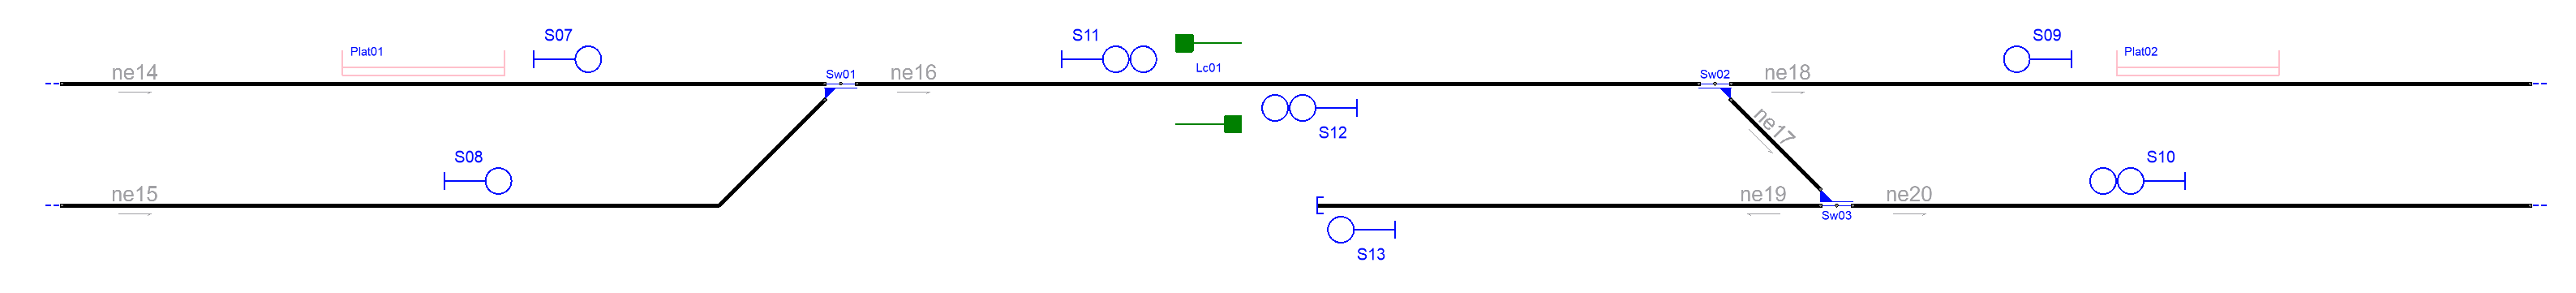
\includegraphics[width=1\textwidth]{resultados-obtenidos/ejemplo2/images/2_original.png}
        \centering\caption{Señalamiento original del ejemplo 2.}
        %\label{fig:LC_P2}
    \end{figure}

    \begin{figure}[h]
        \centering
        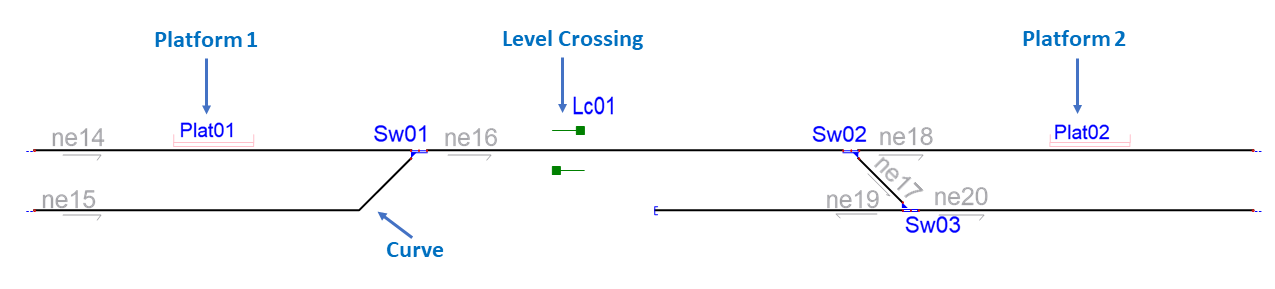
\includegraphics[width=1\textwidth]{resultados-obtenidos/ejemplo2/images/2_empty.png}
        \centering\caption{Topología ferroviaria del ejemplo 2 sin señalamiento.}
        %\label{fig:LC_P2}
    \end{figure}

    \begin{figure}[h]
        \centering
        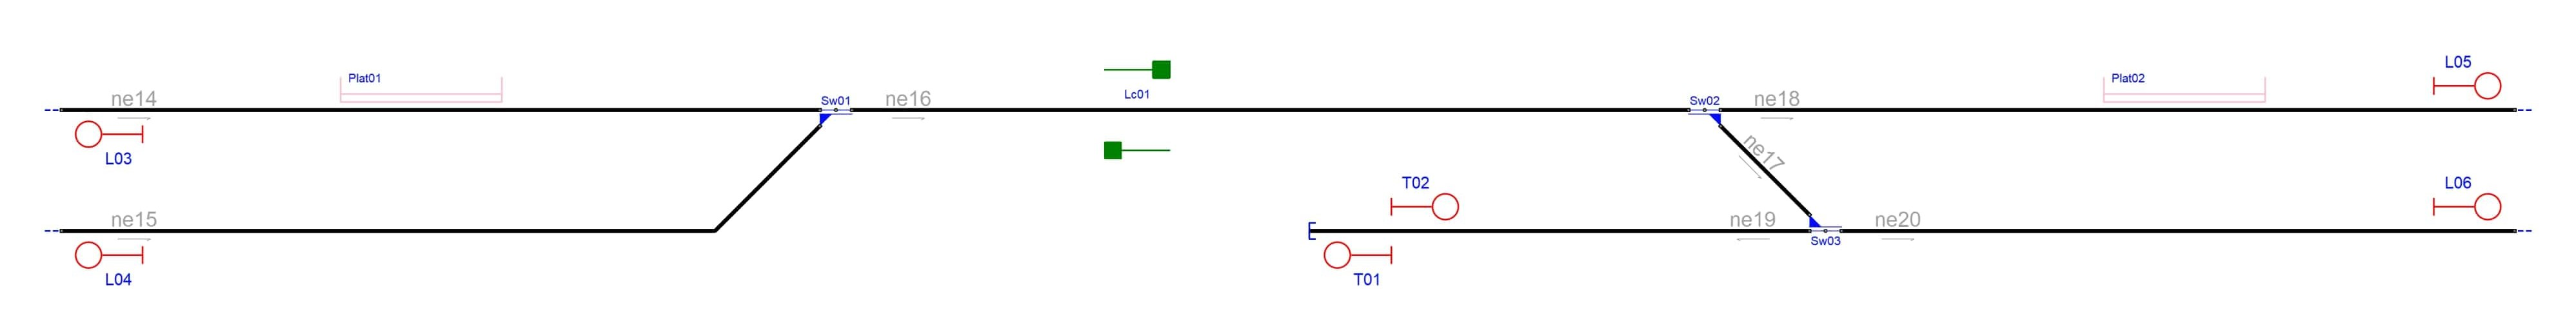
\includegraphics[width=1\textwidth]{resultados-obtenidos/ejemplo2/images/2_step1.png}
        \centering\caption{Señalamiento generado por el RNA para proteger el fín de vía.}
        %\label{fig:LC_P2}
    \end{figure}

    \begin{figure}[h]
        \centering
        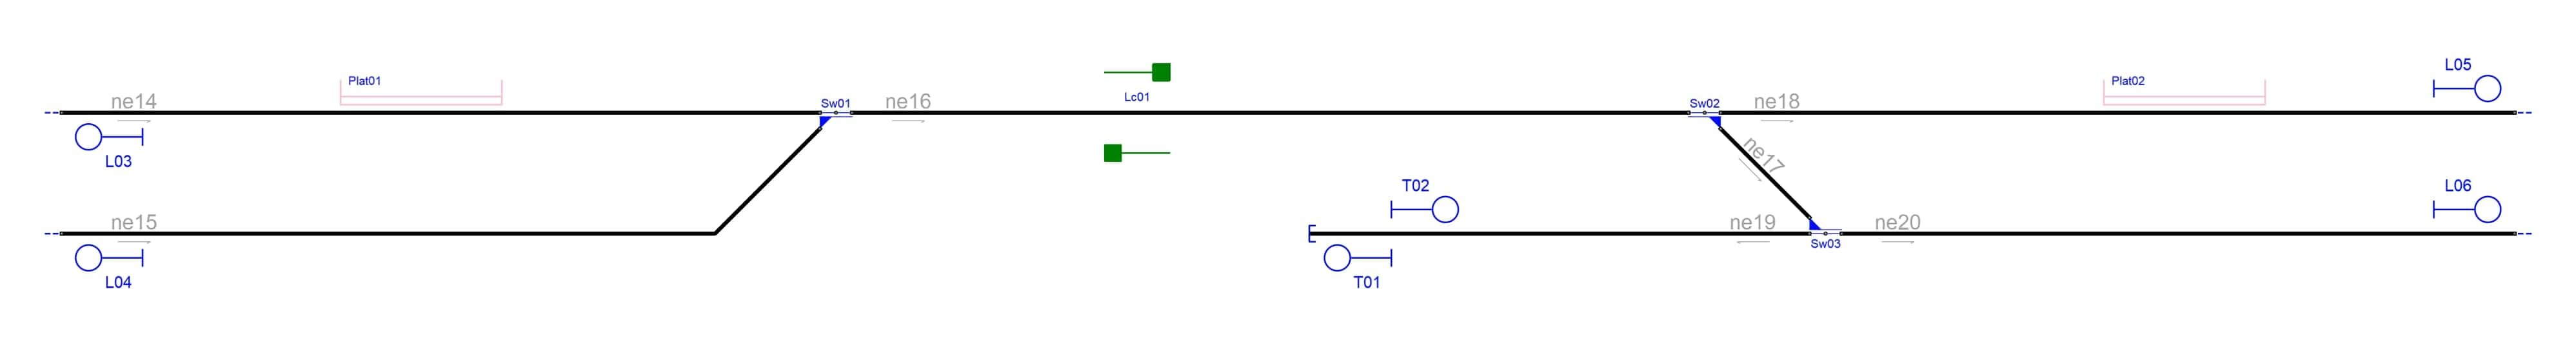
\includegraphics[width=1\textwidth]{resultados-obtenidos/ejemplo2/images/2_step2.png}
        \centering\caption{Señalamiento generado por el RNA para proteger las junturas.}
        %\label{fig:LC_P2}
    \end{figure}

    \begin{figure}[h]
        \centering
        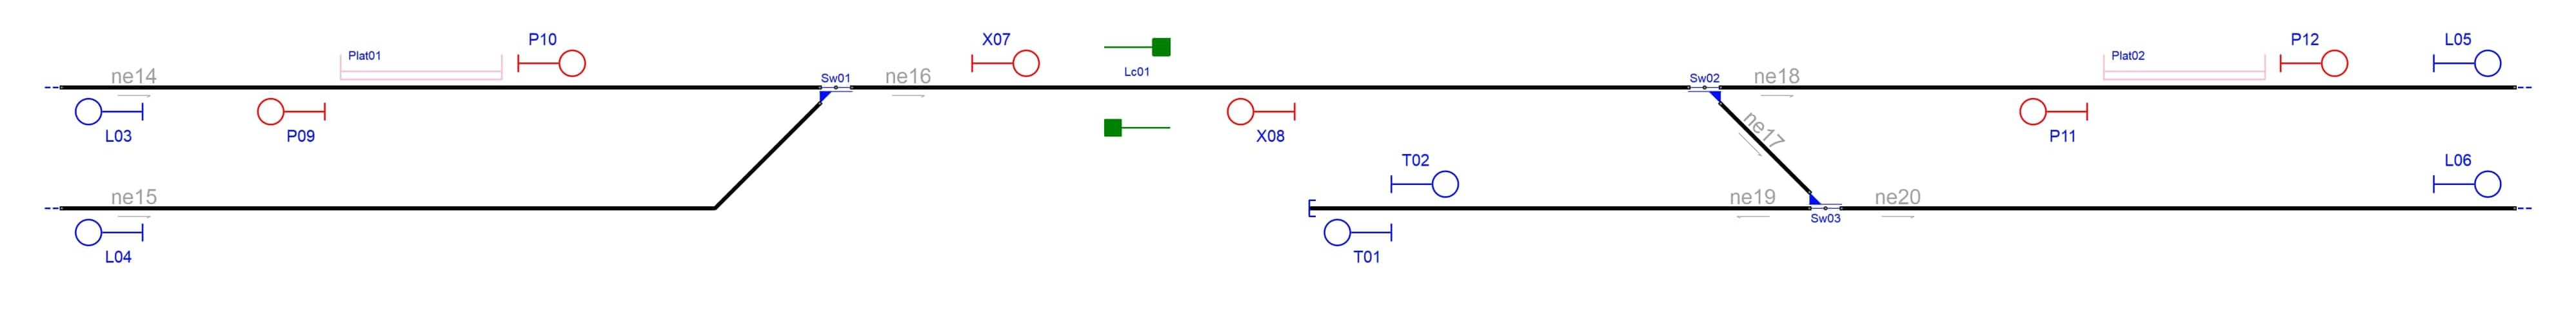
\includegraphics[width=1\textwidth]{resultados-obtenidos/ejemplo2/images/2_step3.png}
        \centering\caption{Señalamiento generado por el RNA para proteger plataformas y cruces de vía.}
        %\label{fig:LC_P2}
    \end{figure}

    \begin{figure}[h]
        \centering
        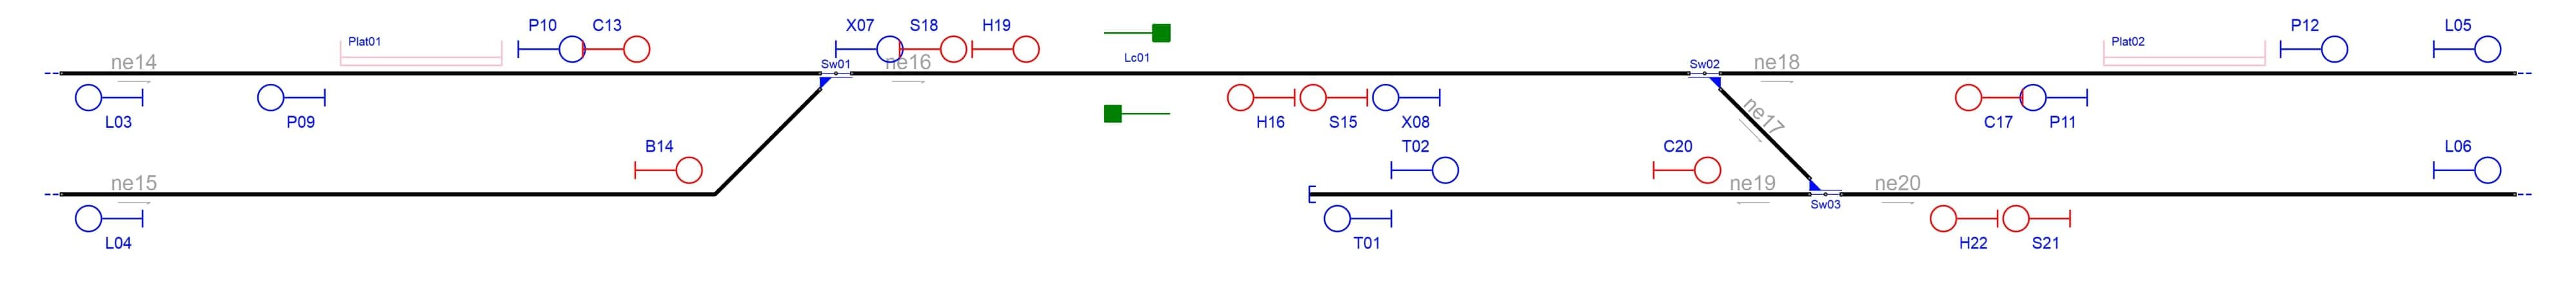
\includegraphics[width=1\textwidth]{resultados-obtenidos/ejemplo2/images/2_step4.png}
        \centering\caption{Señalamiento generado por el RNA para proteger las máquinas de cambios.}
        %\label{fig:LC_P2}
    \end{figure}

    \begin{figure}[h]
        \centering
        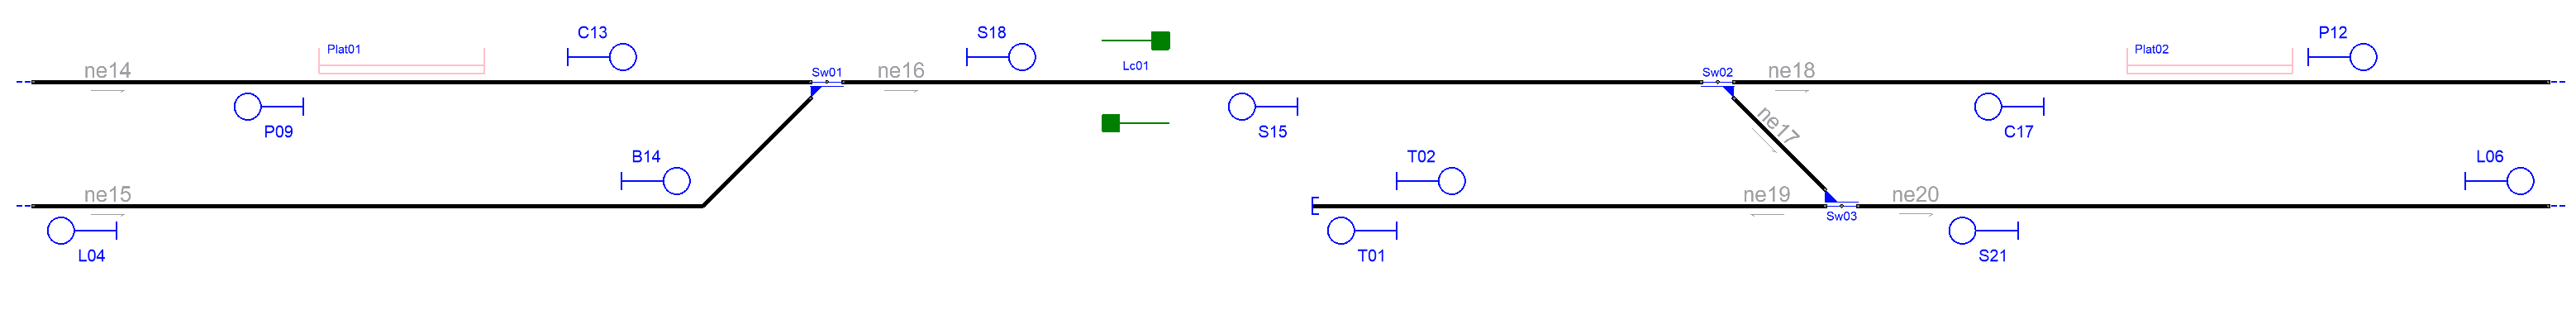
\includegraphics[width=1\textwidth]{resultados-obtenidos/ejemplo2/images/2_RNA.png}
        \centering\caption{Señalamiento generado y simplificado por el RNA.}
        %\label{fig:LC_P2}
    \end{figure}
    
    \subsection{Señalamiento original}

    \lipsum[1]
    
    \begin{table}[H]
        {
        \caption{Tabla de enclavamiento original del ejemplo 2.}
        \label{Tab:tabla_original_2}
        \centering
        \resizebox{1\textwidth}{!}{
            \begin{tabular}{ c c c c c c c }
                \hline	
                    Ruta & Inicio & Final & Cambio & Plataforma & Cruce & netElement \\	
                \hline
                    R$_{01}$  & S$_{07}$ & S$_{11}$ & Sw$_{01}^{N}$ & - & - & ne$_{14}$-ne$_{16}$\\
                    R$_{02}$  & S$_{08}$ & S$_{11}$ & Sw$_{01}^{R}$ & - & - & ne$_{15}$-ne$_{16}$\\
                    R$_{03}$  & S$_{09}$ & S$_{12}$ & Sw$_{02}^{N}$ & - & - & ne$_{18}$-ne$_{16}$\\
                    R$_{04}$  & S$_{10}$ & S$_{13}$ & Sw$_{03}^{N}$ & - & - & ne$_{20}$-ne$_{19}$\\
                    R$_{05}$  & S$_{10}$ & S$_{12}$ & Sw$_{03}^{R}$+Sw$_{02}^{R}$ & - & - & ne$_{20}$-ne$_{17}$-ne$_{16}$\\  
                \hline
            \end{tabular}
        }
     }
    \end{table}
    \section{Señalamiento generado por el RNA}

	El RNA también exporta la misma información mostrada en el Código \ref{lst:EJ2_8} en una hoja de cálculo, similar a la que se visualiza en la Tabla \ref{Tab:tabla_generated_2}.   
    
    \begin{table}[H]
        {
        \caption{Tabla de enclavamiento del ejemplo 2 generada por el RNA.}
        \label{Tab:tabla_generated_2}
        %\centering
        \begin{center}
        \resizebox{0.8\textwidth}{!}{
            \begin{tabular}{ c c c c c c c }
                \hline	
                    Ruta & Inicio & Final & Cambio & Plataforma & Cruce & netElement \\	
                \hline
                    R$_{01}$  & T$_{02}$ & L$_{06}$ & Sw$_{03}^{N}$ & - & - & ne$_{19}$-ne$_{20}$\\
                    R$_{02}$  & C$_{13}$ & S$_{18}$ & Sw$_{01}^{N}$ & - & - & ne$_{14}$-ne$_{16}$\\
                    R$_{03}$  & B$_{14}$ & S$_{18}$ & Sw$_{01}^{R}$ & - & - & ne$_{15}$-ne$_{16}$\\
                    R$_{04}$  & S$_{15}$ & P$_{09}$ & Sw$_{01}^{N}$ & Plat$_{01}$ & Lc$_{01}$ & ne$_{16}$-ne$_{14}$\\
                    R$_{05}$  & S$_{15}$ & L$_{04}$ & Sw$_{01}^{R}$ & Plat$_{01}$ & Lc$_{01}$ & ne$_{16}$-ne$_{15}$\\
                    R$_{06}$  & C$_{17}$ & S$_{15}$ & Sw$_{02}^{N}$ & - & - & ne$_{18}$-ne$_{16}$\\
                    R$_{07}$  & S$_{18}$ & P$_{12}$ & Sw$_{02}^{N}$ & Plat$_{02}$ & Lc$_{01}$ & ne$_{16}$-ne$_{18}$\\
                    R$_{08}$  & S$_{18}$ & L$_{06}$ & Sw$_{02}^{R}$+Sw$_{03}^{R}$ & - & Lc$_{01}$ & ne$_{16}$-ne$_{20}$\\
                    R$_{09}$  & S$_{21}$ & S$_{15}$ & Sw$_{02}^{R}$+Sw$_{03}^{R}$ & - & - & ne$_{20}$-ne$_{16}$\\
                    R$_{10}$  & S$_{21}$ & T$_{01}$ & Sw$_{03}^{N}$ & - & - & ne$_{20}$-ne$_{19}$\\
                \hline
            \end{tabular}
        }
        \end{center}
     }
    \end{table}
    
    En una primera inspección podemos ver que el nuevo señalamiento tiene 10 rutas, versus las 5 rutas del señalamiento original (ver Tabla \ref{Tab:tabla_original_2}). Esto se debe a que todas las vías son consideradas de ambos sentidos por el RNA, lo cuál queda de manifiesto cuando se comprueba que todas las plataformas y cruces de vía son atravesados por al menos una ruta. 
    \subsection{Sistema generado por el ACG}

	En base a la red de grafos, ilustrada en la Figura \ref{fig:EJ2_8}, el ACG determinó la siguiente cantidad de elementos, tal puede visualizarse en el Código \ref{lst:EJ2_8}.
	
	\begin{lstlisting}[language = {}, caption = Cantidad de elementos a implementar por el ACG, label = {lst:EJ2_8}]
	n_netElements:7
	n_switch:3
	n_doubleSwitch:0
	n_borders:4
	n_buffers:1
	n_levelCrossings:1
	n_platforms:2
	n_scissorCrossings:0
	n_signals:12
	N : 45
	M : 38
	\end{lstlisting}
	
	El código VHDL generado por el ACG es importado en un proyecto de Vivado, donde es sintetizado e implementado para generar el bitstream que será utilizado para programar la FPGA. La cantidad de elementos de la FPGA utilizados por el sistema post-síntesis y post-implementación, así como el porcentaje de uso de la plataforma, son detallados en la Tabla \ref{Tab:tabla_ACG_2}.
	
	\begin{table}[H]
		{
			\caption{Síntesis e implementación del ejemplo 2 generado por el ACG.}
			\label{Tab:tabla_ACG_2}
			\centering
			%\small
			%\centering
			\begin{center}
				\resizebox{0.7\textwidth}{!}{
					\begin{tabular}{ c c c c }
						\hline	
						Recursos & Síntesis & Implementación & Uso \\	
						\hline
						LUT & 1881 & 1879 & 3.54\%\\
						FF & 2433 & 2433 & 2.29\%\\
						IO & 16 & 16 & 12.80\%\\
						BUFG & 1 & 1 & 3.13\%\\
						\hline
					\end{tabular}
				}
			\end{center}
		}    
	\end{table}
	
	En este ejemplo, la cantidad de recursos utilizados es baja y el tiempo de sintetización e implementación es de 34 y 35 segundos respectivamente.
    \subsection{Validacion del sistema}

\lipsum[1]

    \begin{table}[H]
        {
        \caption{Equivalencias entre las rutas originales y las generadas por el RNA.}
        \label{Tab:tabla_original_1}
        \centering
        %\small
            %\centering
            \begin{center}
            \resizebox{1\textwidth}{!}{
            \begin{tabular}{ c c c c }
                \hline	
                    Original & Señales & RNA & Señales \\	
                \hline
                    R$_{01}$ & S$_{07}$-S$_{11}$ & R$_{03}$ & B$_{14}$-S$_{18}$ \\
                    R$_{02}$ & S$_{08}$-S$_{11}$ & R$_{06}$ & C$_{17}$-S$_{15}$ \\
                    R$_{03}$ & S$_{09}$-S$_{12}$ & R$_{02}$ & C$_{13}$-S$_{18}$ \\
                    R$_{04}$ & S$_{10}$-S$_{13}$ & R$_{10}$ & S$_{21}$-S$_{15}$ \\
                    R$_{05}$ & S$_{10}$-S$_{12}$ & R$_{09}$ & S$_{21}$-S$_{15}$ \\
                \hline
            \end{tabular}
            }
            \end{center}
        }    
    \end{table}
    
    \lipsum[1]